\documentclass{beamer}

\usepackage{epsfig}
\usepackage{multicol}
\usepackage{geometry}
%\usepackage[dvipsnames]{xcolor}
\usepackage{textcomp}
\usepackage{graphicx}
\usepackage{caption}
\usepackage{subcaption}
\usepackage{amsmath}
\usepackage{tcolorbox}
\usetheme{Boadilla}
\usepackage{pict2e}
\usepackage{tikz}
\usepackage{xcolor}


\title[Traitement du signal numérique]{Traitement du signal numérique - HEI4 IMS}
\author[Antony Bazir]{}

\setlength{\unitlength}{1cm}

\begin{document}
\section{Signal}
\begin{frame}
\frametitle{Introduction}
\textbf{Qu'est ce qu'un signal  ?}

\vspace{1cm}
"\textit{En théorie des systèmes et de l'information, un signal est une quantité mesurable porteuse d’information. "}(fr.wikipedia.org)\\
\vspace{1cm}
\begin{itemize}
\item Porter de l'information : Varier dans le \textbf{temps} et/ ou l'\textbf{espace}
\item Exemples : Images, sons, vidéos, textes, grandeurs électriques, etc..
\end{itemize}
\end{frame}

\begin{frame}
\frametitle{Type de signaux}
\textbf{Comment caractériser un signal ?}\\
\vspace{0.3cm}

\begin{columns}
\column{60mm}
Variation dans le temps et/ou l'espace\\
\includegraphics[scale=0.6]{morse.png} \\
\vspace{1cm}
Dimensionnalité du signal (1D,2D,3D)\\
\includegraphics[scale=0.08]{gauss.png}
\includegraphics[scale=0.08]{gauss2D.png} 
\column{60mm}
Représentation discrète ou continue
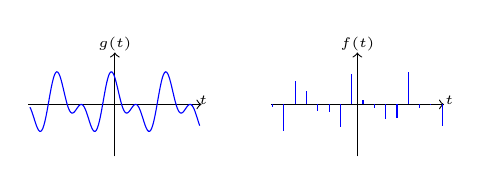
\begin{tikzpicture}
\begin{scope}[scale=0.22]
	\draw[->] (-5,0)-- (5,0);
%\draw (-0.3,-0.3) node {0};
\draw[->] (0,-3)-- (0,3);
\draw (5.1,0.25) node {\tiny $t$};
\draw (0,3.5) node {\tiny $g(t)$};
%\draw (4.5,-0.3) node {1};

\draw[domain=-4.9:4.9,color=blue,samples=160] plot (\x,{2*(0.55*cos(2*\x r)+ 0.45*cos(2*2*(\x+3.14/12) r))});
\end{scope}


\begin{scope}[scale=0.22,xshift=14cm]
	\draw[->] (-5,0)-- (5,0);
%\draw (-0.3,-0.3) node {0};
\draw[->] (0,-3)-- (0,3);
\draw (5.3,0.25) node {\tiny $t$};
\draw (0,3.5) node {\tiny $f(t)$};
%\draw (4.5,-0.3) node {1};


\draw[domain=-4.9:4.9,color=blue,samples=16] plot[ycomb] (\x,{2*(0.55*cos(2*\x r)+ 0.45*cos(2*2*(\x+3.14/12) r))});

\end{scope}
\end{tikzpicture}



\vspace{1cm}
 Déterministe ou aléatoire\\
 \includegraphics[scale=0.1]{gauss.png}
\includegraphics[scale=0.1]{gauss_rand.png} 
\end{columns}
\vspace{0.3cm}

\end{frame}

\begin{frame}
\frametitle{Représentation d'un signal}
Comment représenter synthétiquement l'\textbf{information} contenue dans un signal ?\\
\vspace{0.3cm}
\only<2->{On utilise  des \textbf{fonctions mathématiques} et tous les outils associés\\}

\only<3->{
\vspace{0.3cm}
\underline{Exemple}: $g(t)$, la position du pendule au cours du temps
\begin{center}
\begin{tikzpicture}
\begin{scope}[scale=0.8,xshift=-2cm,yshift=2cm]
\draw (-1,0)-- (1,0);
\draw (0,0)--(-1,-2.4);
\draw (-1,-2.5) circle(0.1);
\draw [->] (-1,-2.5) arc(240:250:4.5);
\end{scope}

\begin{scope}[scale=0.32,xshift=7cm,yshift=2cm]
\draw[->] (-5,0)-- (5,0);
%\draw (-0.3,-0.3) node {0};
\draw[->] (0,-3)-- (0,3);
\draw (5.1,0.25) node {\scriptsize  $t$};
\draw (0,3.5) node {\scriptsize $g(t)$};
\draw (0,-5.1) node{\small $g(t) = cos(t)$};
%\draw (4.5,-0.3) node {1};

\draw[domain=-4.9:4.9,color=blue,samples=160] plot (\x,{2*(0.5*cos(2*\x r)});
\end{scope}
	\end{tikzpicture}
\end{center}
}
\vspace{0.3cm}
\only<4->{Pour traiter un signal, il faut d'abord l'anlayser... Comment ?}
\end{frame}

\begin{frame}
\frametitle{Signaux continus}
Comment analyser les signaux continus ?
\begin{columns}
\column{60mm}
\begin{center}
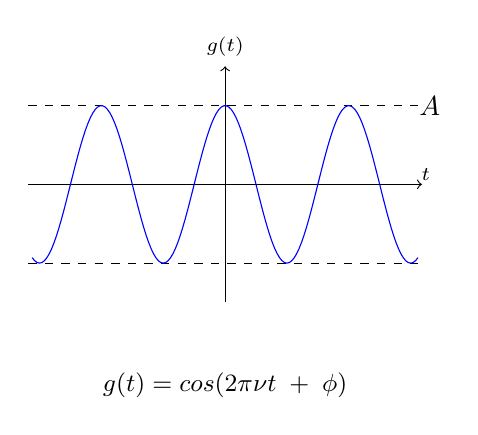
\begin{tikzpicture}
\begin{scope}[scale=0.5]
\draw[->] (-5,0)-- (5,0);
%\draw (-0.3,-0.3) node {0};
\draw[->] (0,-3)-- (0,3);
\draw (5.1,0.25) node {\scriptsize $t$};
\draw (0,3.5) node {\scriptsize $g(t)$};
\draw (0,-5.1) node{\small $g(t) = cos(2\pi \nu t \; + \; \phi)$};
\draw[dashed,thin] (-5,2)--(5,2);
\draw[dashed,thin] (-5,-2)--(5,-2);
\draw (5.2,2) node{$A$};
\draw[domain=-4.9:4.9,color=blue,samples=160] plot (\x,{2*(cos(2*\x r)});
\end{scope}
	\end{tikzpicture}
\end{center}
	
\column{60mm}
Cas d'une fonction sinusoïdale :
\only<2->{
\begin{center}
\begin{itemize}
\item $A$: Amplitude
\vspace{0.5cm}
\item $f$ : Fréquence
\vspace{0.5cm}
\item $\phi$ : Phase
\end{itemize}
\end{center}
}

\only<3->{
\vspace{1cm}
\textbf{Et si la fonction n'est pas une sinusoïde ?}}

\end{columns}
\end{frame}

\begin{frame}
\frametitle{Signaux continus}
On dispose des outils classiques en analyse mathématique: \\
\vspace{0.3cm}
\begin{itemize}
\item Dérivée : $g'(t) =  \frac{d}{dt}g(t)$ (pente locale)
\vspace{0.3cm}
\item Intégrale : $G(t) = \int g(t) dt$ (aire sous la courbe)
\vspace{0.3cm}
\item Norme : $|g(t)| = \sqrt{g(t)^2} $  (distance entre deux points)
\end{itemize}
\vspace{0.3cm}
On peut les appliquer à des \textbf{fonctions (signaux) réelles ou complexes\\}

\only<2->{\vspace{0.3cm}En traitement du signal, on utilise également des \textbf{transformées...}}
\end{frame}

\begin{frame} 
\frametitle{Notion de transformée}
\textbf{Qu'est ce qu'une transformée ?\\}
\vspace{0.5cm}
En mathématique, une transformée fait le lien entre deux fonctions définies dans deux espaces potentiellement différents.\\
\vspace{1cm}
\underline{Exemple}: La transformée de Laplace fait le lien entre une fonction d'une \textbf{variable réelle} et une fonction \textbf{complexe} d'une \textbf{variable complexe.}\\
\vspace{0.5cm}
La transformée de Laplace est une notion centrale en traitement du signal.
\end{frame}

\section{Outils Mathématiques (Laplace et Fourier)}
\subsection{Transformée de Laplace}

\begin{frame}
\frametitle{Transformée de Laplace}
\textbf{Que vous évoque la transformée de Laplace ?}\\

\vspace{1cm}

\only<2->
{
	Transformée de Laplace monolatérale : $L\{f\}(s) = \displaystyle \int^{\infty}_{0} f(t) e^{-st} \; dt$\\ 
	\vspace{0.3cm}
	Transformée de Laplace bilatérale : $L\{f\}(s) = \displaystyle \int^{\infty}_{-\infty} f(t) e^{-st} \; dt$\\
	
\vspace{0.3cm}
avec $t,f(t) \in \mathbb{R}$ et $s,L\{f\}(s) \in \mathbb{C}$\\
\vspace{0.3cm}
}

\only<3-5>
{
Quel type de fonction s'étend toujours de $-\infty$ à $\infty$ ? \only<4-5>{\\ Toutes les fonctions périodiques 
}
}

\only<6->
{
\begin{block}{}
Utile, entre autre, pour analyser des systèmes dynamiques de façon synthétique.
\end{block}
}
\end{frame} 

\begin{frame}
\frametitle{Transformée de Laplace}
En quoi cette transformée impliquant une \textit{intégrale} simplifie-t-elle l'analyse des systèmes ?
\vspace{0.3cm}
\begin{itemize}
\item  Signal "simple" + système "simple" : Laplace peu utile\\
\vspace{0.1cm}
	\hspace{0.2cm}\small{exemple: réponse d'un RC à un échelon de tension}
	\vspace{0.3cm}
\item \normalsize{ Signal ou système "complexe" :}
\begin{itemize}
\item Signal complexe : Décomposition en transitoire/sinusoïdale et sur différentes gammes de fréquences 
\vspace{0.3cm}
\item Système complexe : Décomposition directe en sous-systèmes plus simple
\end{itemize}
\end{itemize}
\vspace{0.3cm}
\textbf{Bien utilisées, la transformée de Laplace et ses dérivées simplifient grandement le traitement de signaux et systèmes "complexes"}
\end{frame}


\begin{frame}
\frametitle{Propriétés de la transformée de Laplace}
Soit $f$ et $g$, deux fonctions de la variable réelle $t$ et $a$ une constante réelle. \\
\vspace{0.3cm}
\begin{itemize}
\item<2-> Linéarité: \only<3->{ $L\{af+g\}(s) = a L\{ f\}(s) + L \{ g \} (s)$}
\vspace{0.4cm}
\item<4-> Dérivation : \only<5->{$ L\{f'\}(s) = \; s L\{f \}(s)$}
\vspace{0.4cm}
\item<5-> Intégration : \only<6->{$ L\{F\}(s) = \frac{\displaystyle 1}{\displaystyle s} L\{f \}(s) $}
\vspace{0.4cm}
\item<7-> Convolution : \only<8->{$ L\{f \star g \} = L\{f \}(s) \cdot L \{ g \} (s)  $}
\end{itemize}

\end{frame}

\begin{frame} 
\frametitle{Produit de convolution}
\underline{Définition}:\\
$(f \star g) (x) =  \displaystyle \int^{\infty}_{-\infty} f(x-t)g(t) \; dt  =  \displaystyle \int^{\infty}_{-\infty}  f(t)g(x-t)  \; dt $ \\
\vspace{0.2cm}
Illustrons avec deux fonctions porte de même largeur \\
\vspace{0.2cm}

\begin{columns}
\column{60mm}
\begin{center}
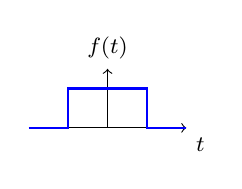
\begin{tikzpicture}
\begin{scope}[scale=0.5]
\draw[->] (0,0)  -- (0,1.5)node[above] {\footnotesize{$f(t)$}};
\draw[->] (-2,0)-- (2,0) node[below right] {\footnotesize{$t$}};

\draw[thick,blue] (-2,0)--(-1,0)--(-1,1)--(1,1)--(1,0)--(2,0);
\end{scope}
\end{tikzpicture}
\end{center}
\only<1>{
\begin{center}
\begin{tikzpicture}
\begin{scope}[scale=0.5]
\draw[->] (0,0)  -- (0,1.5)node[above] {\footnotesize{$f, g$}};
\draw[->] (-5,0)-- (5,0) node[below right] {\footnotesize{$t$}};

\draw[thick,blue] (-2,0)--(-1,0)--(-1,1)--(1,1)--(1,0)--(2,0);
\draw[thick,red] (-2-3,0)--(-1-3,0)--(-1-3,1)--(1-3,1)--(1-3,0)--(2-3,0);
\draw (0,-0.75) node{\small{$x<-2$}};
\end{scope}

\end{tikzpicture}
\end{center}
}

\only<2>{
\begin{center}
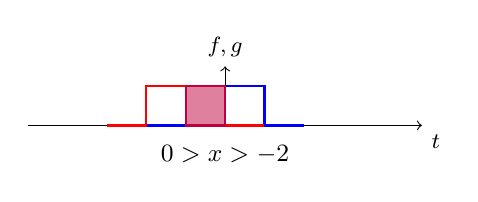
\begin{tikzpicture}
\begin{scope}[scale=0.5]
\draw[->] (0,0)  -- (0,1.5)node[above] {\footnotesize{$f, g$}};
\draw[->] (-5,0)-- (5,0) node[below right] {\footnotesize{$t$}};

\draw[thick,blue] (-2,0)--(-1,0)--(-1,1)--(1,1)--(1,0)--(2,0);
\draw[thick,red] (-2-1,0)--(-1-1,0)--(-1-1,1)--(1-1,1)--(1-1,0)--(2-1,0);
\draw[thick,purple,fill=purple!50!white] (-1,0) rectangle (0,1) ;
\draw (0,-0.75) node{\small{$0>x>-2$}};
\end{scope}

\end{tikzpicture}
\end{center}
}

\only<3>{
\begin{center}
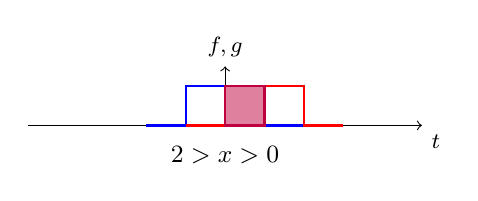
\begin{tikzpicture}
\begin{scope}[scale=0.5]
\draw[->] (0,0)  -- (0,1.5)node[above] {\footnotesize{$f, g$}};
\draw[->] (-5,0)-- (5,0) node[below right] {\footnotesize{$t$}};

\draw[thick,blue] (-2,0)--(-1,0)--(-1,1)--(1,1)--(1,0)--(2,0);
\draw[thick,red] (-2+1,0)--(-1+1,0)--(-1+1,1)--(1+1,1)--(1+1,0)--(2+1,0);
\draw[thick,purple,fill=purple!50!white] (0,1) rectangle (1,0) ;
\draw (0,-0.75) node{\small{$2>x>0$}};
\end{scope}

\end{tikzpicture}
\end{center}
}


\only<4>{
\begin{center}
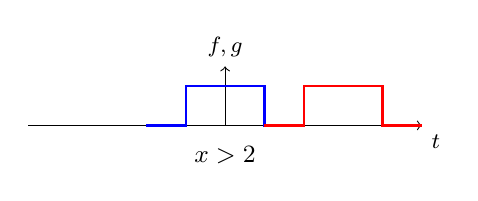
\begin{tikzpicture}
\begin{scope}[scale=0.5]
\draw[->] (0,0)  -- (0,1.5)node[above] {\footnotesize{$f, g$}};
\draw[->] (-5,0)-- (5,0) node[below right] {\footnotesize{$t$}};

\draw[thick,blue] (-2,0)--(-1,0)--(-1,1)--(1,1)--(1,0)--(2,0);
\draw[thick,red] (-2+3,0)--(-1+3,0)--(-1+3,1)--(1+3,1)--(1+3,0)--(2+3,0);
%\draw[thick,purple,fill=purple!50!white] (0,1) rectangle (1,0) ;
\draw (0,-0.75) node{\small{$x>2$}};
\end{scope}

\end{tikzpicture}
\end{center}
}
\column{60mm}
\begin{center}
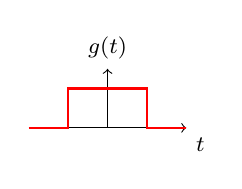
\begin{tikzpicture}
\begin{scope}[scale=0.5]
\draw[->] (0,0) -- (0,1.5)node[above] {\footnotesize{$g(t)$}};
\draw[->] (-2,0)-- (2,0) node[below right] {\footnotesize{$t$}};

\draw[thick,red] (-2,0)--(-1,0)--(-1,1)--(1,1)--(1,0)--(2,0);

\end{scope}
\end{tikzpicture}
\end{center}
\only<1>{
\begin{center}
\begin{tikzpicture}
\begin{scope}[scale=0.5]
\draw[->] (0,0) -- (0,1.5)node[above] {\footnotesize{$f\star g$}};
\draw[->] (-5,0)-- (5,0) node[below right] {\footnotesize{$x$}};

\draw[thick,red!50!blue] (-5,0)--(-2,0);
%--(-1,1)--(1,1)--(1,0)--(2,0);

\end{scope}
\end{tikzpicture}
\end{center}
}

\only<2>{
\begin{center}
\begin{tikzpicture}
\begin{scope}[scale=0.5]
\draw[->] (0,0) -- (0,1.5)node[above] {\footnotesize{$f\star g$}};
\draw[->] (-5,0)-- (5,0) node[below right] {\footnotesize{$x$}};

\draw[thick,red!50!blue] (-5,0)--(-2,0)--(0,1);
%--(-1,1)--(1,1)--(1,0)--(2,0);

\end{scope}
\end{tikzpicture}
\end{center}
}

\only<3>{
\begin{center}
\begin{tikzpicture}
\begin{scope}[scale=0.5]
\draw[->] (0,0) -- (0,1.5)node[above] {\footnotesize{$f\star g$}};
\draw[->] (-5,0)-- (5,0) node[below right] {\footnotesize{$x$}};

\draw[thick,red!50!blue] (-5,0)--(-2,0)--(0,1)--(2,0);
%--(2,0);
%--(-1,1)--(1,1)--(1,0)--(2,0);

\end{scope}
\end{tikzpicture}
\end{center}
}

\only<4>{
\begin{center}
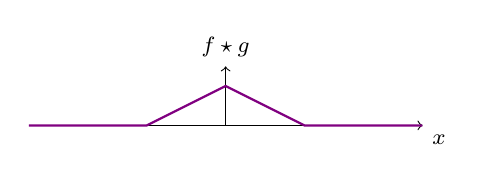
\begin{tikzpicture}
\begin{scope}[scale=0.5]
\draw[->] (0,0) -- (0,1.5)node[above] {\footnotesize{$f\star g$}};
\draw[->] (-5,0)-- (5,0) node[below right] {\footnotesize{$x$}};

\draw[thick,red!50!blue] (-5,0)--(-2,0)--(0,1)--(2,0)--(5,0);

\end{scope}
\end{tikzpicture}
\end{center}
}
\end{columns}
\end{frame} 

\begin{frame} 
\frametitle{Produit de convolution}
\underline{Définition}:\\
$(f \star g) (x) =  \displaystyle \int^{\infty}_{-\infty} f(x-t)g(t) \; dt  =  \displaystyle \int^{\infty}_{-\infty}  f(t)g(x-t)  \; dt $ \\
\vspace{0.2cm}

\begin{columns}
\column{60mm}

\begin{center}
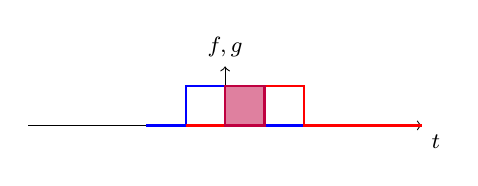
\begin{tikzpicture}
\begin{scope}[scale=0.5]
\draw[->] (0,0)  -- (0,1.5)node[above] {\footnotesize{$f, g$}};
\draw[->] (-5,0)-- (5,0) node[below right] {\footnotesize{$t$}};

\draw[thick,blue] (-2,0)--(-1,0)--(-1,1)--(1,1)--(1,0)--(2,0);
\draw[thick,red] (-2+1,0)--(-1+1,0)--(-1+1,1)--(1+1,1)--(1+1,0)--(2+3,0);
\draw[thick,purple,fill=purple!50!white] (0,1) rectangle (1,0) ;
\end{scope}

\end{tikzpicture}
\end{center}

\column{60mm}

\begin{center}
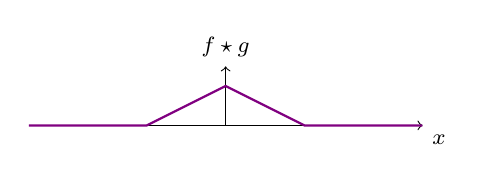
\begin{tikzpicture}
\begin{scope}[scale=0.5]
\draw[->] (0,0) -- (0,1.5)node[above] {\footnotesize{$f \star g$}};
\draw[->] (-5,0)-- (5,0) node[below right] {\footnotesize{$x$}};

\draw[thick,red!50!blue] (-5,0)--(-2,0)--(0,1)--(2,0)--(5,0);

\end{scope}
\end{tikzpicture}
\end{center}
\end{columns}

\begin{itemize}
\item On calcule l'aire sous le croisement des courbes pour chaque point $x$
\end{itemize}
\vspace{0.4cm}
\begin{block}{}
Le produit de convolution est une opération fondamentale en théorie des systèmes et traitement du signal
\end{block}
\end{frame} 

\begin{frame}
\frametitle{Produit de convolution}
\begin{columns}
\column{60mm}
\includegraphics[scale=0.4]{Convolution_Illustrated.png}\\
\footnotesize{\textit{Illustration de la convolution (wikipedia.org)}}
\column{60mm}
\begin{itemize}
\item PSF : \textbf{Réponse impulsionnelle} d'un système d'imagerie 
\vspace{0.3cm}
\item Utile pour reconstruire le "véritable" objet
\vspace{0.3cm}
\item Cadre théorique largement utilisée en imagerie numérique
\end{itemize}
\end{columns}
\end{frame}

\begin{frame}
\frametitle{Produit de convolution}
\begin{columns}
\column{60mm}
\includegraphics[scale=0.4]{Convolution_Illustrated.png}\\
\footnotesize{\textit{Illustration de la convolution (wikipedia.org)}}\\
\vspace{0.2cm}
\includegraphics[scale=0.3]{olympus.jpg}\\
\footnotesize{\textit{Utilisation de la déconvolution (olympus-lifescience.com)}}\\
\column{60mm}
\begin{itemize}
\item PSF : \textbf{Réponse impulsionnelle} d'un système d'imagerie 
\vspace{0.3cm}
\item Utile pour reconstruire le "véritable" objet
\vspace{0.3cm}
\item Cadre théorique largement utilisée en imagerie numérique
\end{itemize}
\end{columns}
\end{frame}


\begin{frame} 
\frametitle{Transformée de Laplace}

\textbf{Exercice: Calculer les transformées de Laplace suivantes}\\
\vspace{0.3cm}
Rappel : $L\{f\}(s) = \displaystyle \int^{\infty}_{-\infty} f(t) e^{-st} \; dt$
\vspace{0.3cm}
\begin{itemize}
\item $u(t)$ (échelon de heaviside)
\vspace{0.2cm}
\item $r(t) = t$ (rampe)
\vspace{0.2cm}
\item $f(t) = e^{-at}$ (exponentielle décroissante)
\vspace{0.2cm}
\item $\delta (t)$ (impulsion de dirac) 
%\vspace{0.2cm}
%\item $sin(\omega_0 t)$
\end{itemize}

\end{frame} 

\begin{frame} 
\frametitle{Transformée de Laplace}

\textbf{Exercice: Calculer les transformées de Laplace suivantes}\\
\vspace{0.3cm}
Rappel : $L\{f\}(s) = \displaystyle \int^{\infty}_{-\infty} f(t) e^{-st} \; dt$
\vspace{0.3cm}
\begin{itemize}
\item $u(t)$  \only<2->{$\rightarrow \frac{\displaystyle 1}{\displaystyle s} $} 
\vspace{0.2cm}
\item $r(t) = t$  \only<3->{$\rightarrow \frac{\displaystyle 1}{ \displaystyle s^2} $}
\vspace{0.2cm}
\item $f(t) = e^{-at}$  \only<4->{$\rightarrow \frac{\displaystyle 1}{\displaystyle p+a} $}
\vspace{0.2cm}
\item $\delta (t)$ \only<5->{$\rightarrow 1$} 
%\vspace{0.2cm}
%\item $sin(\omega t)$  \only<6->{$\rightarrow \frac{\displaystyle \omega_0^2}{ \displaystyle p^2 + \omega_0^2} $}
\end{itemize}

\end{frame}

\subsection{Transformée de Fourier et lien avec la transformée de Laplace}

\subsubsection{Transformée de Fourier}


\begin{frame}
\frametitle{Transformée de Fourier}
\textbf{Question: Quelle est pour vous le lien entre transformée de Laplace et transformée de Fourier ?}\\
\vspace{1 cm}
\only<2->
{
\begin{center}
	$L\{f\}(s) = \displaystyle \int^{\infty}_{-\infty} f(t) e^{-st} \; dt $ \only<3->{$ \rightarrow TF\{ f \}(\nu) = \displaystyle \int^{\infty}_{-\infty} f(t) e^{-j2\pi \nu t} dt $}
\end{center} 
}

\only<4->{
\begin{block}{}
La transformée de Fourier peut s'écrire comme un cas particulier de la transformée de Laplace bilatérale.
\end{block}
}
\end{frame}

\begin{frame}
\frametitle{Transformée de Fourier}
Quand/Comment s'utilise la transformée de Fourier ?\\
\vspace{0.5cm}
La variable de Laplace s'écrit $s \;\; = \;\; a + j \omega \;\; = \;\; a + j 2\pi \nu  $\\
\vspace{0.3cm}
\begin{itemize}
\item La partie réelle $a$ décrit le régime transitoire du système
\item La partie imaginaire $\omega = 2\pi \nu$ décrit le régime "permanent" 
\end{itemize} 
\vspace{0.3cm}
Le régime permanent correspond à des \textbf{excitations sinusoïdales/périodiques\\
}
\vspace{0.5cm}
\textbf{La variable de fourier $j2\pi \nu$ correspond à la partie imaginaire de la variable de Laplace}
\end{frame}

\begin{frame}
\frametitle{Transformée de Fourier}
\begin{columns}
\column{60mm}
Transformée de Laplace : 
\vspace{0.4cm}
\begin{itemize} 
\item $s = a + j 2 \pi \nu$
\vspace{0.4cm}
\item régime transitoire ET permanent
\end{itemize}
\column{60mm}
Transformée de Fourier :
\vspace{0.4cm}
\begin{itemize}
\item $j 2 \pi \nu$ 
\vspace{0.4cm}
\item  régime permanent 
\end{itemize}
\end{columns}
\vspace{1cm}
La \textbf{transformée  de Fourier} sert pour les systèmes où on ne s'intéresse pas \textbf{au régime transitoire}\\
\end{frame}

\begin{frame}
\frametitle{Transformée de Fourier}
La \textbf{transformée  de Fourier} sert pour les systèmes où on ne s'intéresse pas \textbf{au régime transitoire}\\
\vspace{0.5cm}
\underline{Exemple:} Mécanique Vibratoire \\
\center
\includegraphics[scale=0.4]{Tacoma.jpg}\\
\footnotesize{Pont du Tacoma effondré après une mise en \textbf{résonance} due au vent}
\end{frame}

\subsubsection{Spectre}
\begin{frame}
\frametitle{Transformée de Fourier}
\[ TF\{ f \}(\nu) = \displaystyle \int^{\infty}_{-\infty} f(t) \; e^{-j2\pi \nu t} dt   = F(\nu) \]\\
\vspace{1cm}

La fonction $F(\nu)$ est généralement désignée comme \textbf{spectre fréquentiel} de $f(t)$ \\

\vspace{1cm}
\only<2->{
\underline{Note}: $F(\nu)$ est une fonction \textbf{complexe} 
}

\only<3->{
\begin{block}{}
Comment le représenter ? 
\end{block}
}
\end{frame}

\begin{frame}
\frametitle{Transformée de Fourier : Spectre }

Comment représenter $F(\nu)$  ? \\

\vspace{1cm} 

2 possibilités pour représenter un nombre complexe $z$: \\
\vspace{0.2cm}

\begin{itemize}
\item $z = a+ ib$
\vspace{0.4cm}
\item $z = r\cdot e^{i \theta}$
\end{itemize} 

\vspace{0.7 cm}

\only<2->{
\begin{block}{}
Dans la grande majorité des cas, c'est la représentation module/argument $z = r\cdot e^{i \theta}$ qui est utilisée.
\end{block}
}




\end{frame} 

\begin{frame}
\frametitle{Module et phase d'un nombre complexe}


Soit un nombre complexe $z = a +ib$, alors \\
\vspace{0.3cm}
\only<2->{ \underline{Module}: \\
$|z|=r = \sqrt{a^2 + b^2}$\\
\vspace{0.3cm}}



\only<3->{\underline{Phase }:\\
 $\text{arg}(z) = \theta = \arctan(\frac{\displaystyle b}{\displaystyle a})$}

\vspace{0.7cm}
\only<4->
{
On va prendre la fonction $g_1(t) = \cos(2 t)$ pour illustrer
}
\end{frame}

\subsubsection{Module et phase: exemples}


\begin{frame}
\frametitle{Transformée  de Fourier : Spectre}
Soit $g_1(t) = \cos(2 t)$ \\

\only<2->{
\begin{center}
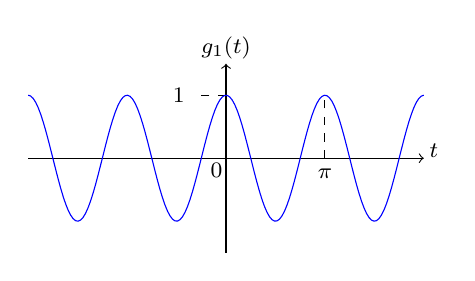
\begin{tikzpicture}
\begin{scope}[scale=0.4]
	\draw[->] (-6.28,0)-- (6.28,0);
\draw (-0.3,-0.4) node {\footnotesize{0}};
\draw[->] (0,-3)-- (0,3);
\draw (2.1*pi,0.25) node {\footnotesize{$t$}};
\draw (0,3.5) node {\footnotesize{$g_1(t)$}};
\draw[dashed] (0,2)--(-1,2);
\draw (-1.5,2) node{\footnotesize{1}};
\draw[dashed] (3.14,0)--(3.14,2);
\draw (3.14,-0.5) node{\footnotesize{$\pi$}}; 

\draw[domain=-6.28:6.28,color=blue,samples=160] plot (\x,{2*cos(2*\x r)});	
\end{scope}
\end{tikzpicture}
\end{center}
}


\vspace{0.3 cm} 

\only<3->{
 $$TF\{ g_1 \}(\nu) = \int^{\infty}_{-\infty} \cos(2t) \; e^{-2\pi j \nu t} \; dt$$ \only<4->{$$= \frac{\displaystyle \delta(\nu - 1/\pi) + \delta(\nu + 1/\pi)}{\displaystyle 2}
$$}}

\end{frame}

\begin{frame}
\frametitle{Transformée  de Fourier : Spectre}
\small{Expression du \textbf{spectre} de $g_1$ (fonction complexe)}
 $$TF\{ g_1 \}(\nu) = \int^{\infty}_{-\infty} g_1(t) \; e^{-2\pi j \nu t} \; dt= \frac{\displaystyle \delta(\nu - 1/\pi) + \delta(\nu + 1/\pi)}{\displaystyle 2}$$\\
 

 
 \vspace{1cm}
 \underline{Module}:
 \only<2->{
 $$|TF\{ g_1 \}(\nu)| = |G_1(\nu)| = \frac{\displaystyle \delta(\nu - 1/\pi) + \delta(\nu + 1/\pi)}{\displaystyle 2} $$
 }
 
\only<3->{
\begin{center}
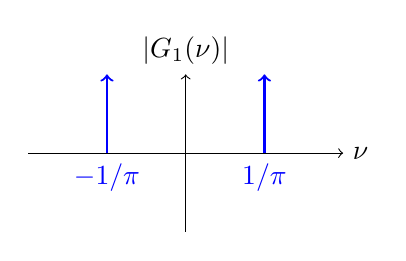
\begin{tikzpicture}
\draw[->] (-2,0)--(2,0) node[right]{$\nu$};
\draw[->] (0,-1)--(0,1) node[above]{$|G_1(\nu)|$};
\draw[->,blue,thick] (-1,0) node[below]{$-1/\pi$}--(-1,1) ;
\draw[->,blue,thick] (1,0) node[below]{$1/\pi$}--(1,1) ;
\end{tikzpicture}
\end{center}
}
\end{frame}

\begin{frame}
\frametitle{Transformée de Fourier : Spectre}
$$G_1(\nu) = \frac{\displaystyle \delta(\nu - 1/\pi) + \delta(\nu + 1/\pi)}{\displaystyle 2} $$\\

\vspace{0.6cm}
\underline{Phase}:
\only<2->{
$$arg(G_1(\nu)) = $$ \only<3->{ $$\arctan\left(\frac{0}{\frac{\displaystyle \delta(\nu - 1/\pi) + \delta(\nu + 1/\pi)}{\displaystyle 2}}\right) = 0$$}\\
}
\vspace{0.3cm}
\only<3->{
\begin{center}
\begin{tikzpicture}
\draw[->] (-2,0)--(2,0) node[right]{$\nu$};
\draw[->] (0,-1)--(0,1) node[above]{$\text{arg}(G_1(\nu))$};
\draw[->,blue,thick] (-1,0) node[below]{$-1/\pi$}--(-1,0) ;
\draw[->,blue,thick] (1,0) node[below]{$1/\pi$}--(1,0) ;
\end{tikzpicture}
\end{center}
}

\end{frame}

\begin{frame}
\frametitle{Transformée  de Fourier : Spectre}
En résumé, \\
\vspace{0.3cm}
\[g_1(t) = \cos(2 t) \rightarrow  G_1(\nu) = \frac{\displaystyle \delta(\nu - 1/\pi) + \delta(\nu + 1/\pi)}{\displaystyle 2} \]

\begin{columns}
\column{60mm}
\only<2->{
\underline{Module}:\\
\[|G_1(\nu)| = \frac{\displaystyle \delta(\nu - 1/\pi) + \delta(\nu + 1/\pi)}{\displaystyle 2}\]\\
}
\vspace{0.1cm}
\only<3->
{
\begin{center}
\begin{tikzpicture}
\draw[->] (-2,0)--(2,0) node[right]{$\nu$};
\draw[->] (0,-1)--(0,1) node[above]{$|G_1(\nu)|$};
\draw[->,blue,thick] (-1,0) node[below]{\scriptsize $-1/\pi$}--(-1,1) ;
\draw[->,blue,thick] (1,0) node[below]{\scriptsize $1/\pi$}--(1,1) ;
\end{tikzpicture}
\end{center}
}

\column{60mm}
\only<2->{
\underline{Phase}:\\
$$arg(G_1(\nu))  = 0 $$ \\
}
\vspace{0.65cm}
\only<3->
{
\begin{center}
\begin{tikzpicture}
\draw[->] (-2,0)--(2,0) node[right]{\footnotesize{$\nu$}};
\draw[->] (0,-1)--(0,1) node[above]{\footnotesize{$\text{arg}(G_1(\nu))$}};
\draw[->,blue,thick] (-1,0) node[below]{\scriptsize $-1/\pi$}--(-1,0) ;
\draw[->,blue,thick] (1,0) node[below]{ \scriptsize $1/\pi$}--(1,0) ;
\end{tikzpicture}
\end{center}
}
\end{columns}
\end{frame}

\begin{frame}
\frametitle{Transformée  de Fourier : Spectre}
Spectre de $g_2(t) = 0.55\cos(2 t) + 0.45 \cos(4 t + \frac{\pi}{3})$ \\
\only<2->{
\begin{center}
\begin{tikzpicture}
\begin{scope}[scale=0.3,xshift=-12cm]
	\draw[->] (-6.28,0)-- (6.28,0);
%\draw (-0.3,-0.3) node {0};
\draw[->] (0,-3)-- (0,3);
\draw (2*pi+0.2,0.25) node {\scriptsize  $t$};
\draw (0,3.5) node {\scriptsize $ 0.55\cos(2 t)$};
%\draw (4.5,-0.3) node {1};

		\draw[domain=-6.28:6.28,color=orange,dashed,samples=160] plot (\x,{2*(0.55*cos(2*\x r))});
	\end{scope}
	
	\begin{scope}[scale=0.3,xshift=12cm]
	\draw[->] (-6.28,0)-- (6.28,0);
%\draw (-0.3,-0.3) node {0};
\draw[->] (0,-3)-- (0,3);
\draw (2*pi+0.2,0.25) node {\scriptsize $t$};
\draw (0,3.5) node {\scriptsize $0.45 \cos(4 t + \frac{\pi}{3})$};
%\draw (4.5,-0.3) node {1};

		\draw[domain=-6.28:6.28,color=orange,dashed,samples=160] plot (\x,{2*(0.45*cos(2*2*(\x+3.14/12) r))});
	\end{scope}
	
\begin{scope}[scale=0.4,yshift=-6cm]
	\draw[->] (-6.28,0)-- (6.28,0);
%\draw (-0.3,-0.3) node {0};
\draw[->] (0,-3)-- (0,3);
\draw (2*pi+0.2,0.25) node {\scriptsize $t$};
\draw (0,3.5) node {\scriptsize $g_2(t)$};
%\draw (4.5,-0.3) node {1};

		\draw[domain=-6.28:6.28,color=orange,samples=160] plot (\x,{2*(0.55*cos(2*\x r)+ 0.45*cos(2*2*(\x+3.14/12) r))});
	\end{scope}
	\end{tikzpicture}
\end{center}
}
\end{frame}

\begin{frame}
\frametitle{Transformée  de Fourier : Spectre}

\[ TF\{ g_2 \}(f) = G_2(\nu)\]\\
\[ =   \frac{0.55}{2}(\delta(\nu+1/\pi) + \delta(\nu-1/\pi)) + \frac{0.45}{2}(\delta(\nu+2/\pi) + \delta(\nu-2/\pi)) \cdot e^{2 j \pi \frac{\pi}{3} \nu }\]\\

\vspace{0.5 cm}

\[|G_2(\nu)| = \bigl[(\frac{0.55}{2}(\delta(\nu+1/\pi) + \delta(\nu-1/\pi))+ \] \\
\[ \frac{0.45}{2}(\delta(\nu+2/\pi) + \delta(\nu-2/\pi)) \cdot  \cos(2\frac{\pi^2}{3} \nu))^2 \]\\
\[+(\frac{0.45}{2}(\delta(\nu+2/\pi) + \delta(\nu-2/\pi)) \cdot  \sin(2\frac{\pi^2}{3} \nu))^2 \bigr] ^{1/2} \]

\end{frame}

\begin{frame} 
\frametitle{Transformée  de Fourier : Spectre}

\[|G_2(\nu)| = \bigl[(\frac{0.55}{2}(\delta(\nu+1/\pi) + \delta(\nu-1/\pi))+  \] \\
\[ \frac{0.45}{2}(\delta(\nu+2/\pi) + \delta(\nu-2/\pi)) \cdot  \cos(2\frac{\pi^2}{3} \nu))^2 \]\\
\[+(\frac{0.45}{2}(\delta(\nu+2/\pi) + \delta(\nu-2/\pi)) \cdot  \sin(2\frac{\pi^2}{3} \nu))^2 \bigr] ^{1/2} \]\\

\vspace{0.5cm}
\only<2->{
\begin{center}
\begin{tikzpicture}
\draw[->] (-2.5,0)--(2.5,0) node[right]{\footnotesize{$\nu$}};
\draw[->] (0,-1)--(0,1) node[above]{\footnotesize{$|G_2(\nu)|$}};
\draw[->,orange,thick] (-1,0) node[below]{\scriptsize $-1/\pi$}--(-1,0.55) ;
\draw[->,orange,thick] (1,0) node[below]{\scriptsize $1/\pi$}--(1,0.55) ;
\draw[->,orange,thick] (-2,0) node[below]{\scriptsize $-2/\pi$}--(-2,0.225) ;
\draw[->,orange,thick] (2,0) node[below]{\scriptsize $2/\pi$}--(2,0.225) ;
\end{tikzpicture}
\end{center}
}
\end{frame}

\begin{frame}
\frametitle{Transformée  de Fourier : Spectre}
\[ arg(G_2(\nu)) = \]\\
\[ \arctan \left( \frac{\frac{0.45}{2}(\delta_2) \cdot  \sin(2\frac{\pi^2}{3} \nu)}{\frac{0.55}{2}(\delta_1)+
 \frac{0.45}{2}(\delta_2) \cdot  \cos(2\frac{\pi^2}{3} \nu)} \right) \]\\
 \vspace{0.3cm} 
 \only<2->{
 \[\text{arg}(G_2(\nu)) = 2\frac{\pi^2}{3} \nu \cdot \frac{0.45}{2}(\delta(\nu+2/\pi) + \delta(\nu-2/\pi)) \]\\
 }

 \vspace{0.3cm}
 
 \only<3->
{
\begin{center}
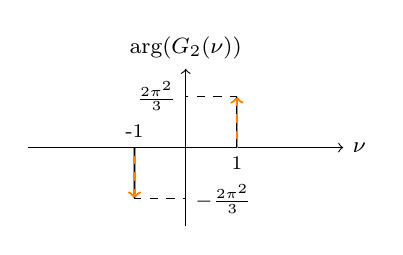
\begin{tikzpicture}
\draw[->] (-2,0)--(2,0) node[right]{\footnotesize{$\nu$}};
\draw[->] (0,-1)--(0,1) node[above]{\footnotesize{$\text{arg}(G_2(\nu))$}};
%\draw[orange,thick] (-1,-1) --(1,1) ;
\draw[->,orange,thick] (-0.65,0)--(-0.65,-0.65) ;
\draw[->,orange,thick] (0.65,0)--(0.65,0.65) ;
\draw[dashed] (-0.65,0)node[above]{\scriptsize -1} --(-0.65,-0.65)--(0,-0.65)node[right]{\scriptsize $-\frac{2\pi^2}{3}$} ;
\draw[dashed] (0.65,0)node[below]{\scriptsize 1} --(0.65,0.65)--(0,0.65)node[left]{\scriptsize $\frac{2\pi^2}{3}$} ;
\end{tikzpicture}
\end{center}
}
\end{frame}

\begin{frame}
\frametitle{Transformée  de Fourier : Spectre}
\[ TF\{ g_2 \}(f) = G_2(\nu)\]\\
\[ =   \frac{0.55}{2}(\delta(\nu+1/\pi) + \delta(\nu-1/\pi)) + \frac{0.45}{2}(\delta(\nu+2/\pi) + \delta(\nu-2/\pi)) \cdot e^{2 j \pi \frac{\pi}{3} \nu }\]\\

\vspace{0.3cm}
%addd more steps here
\begin{columns}
\column{60mm}
\only<2->{
\begin{center}
\begin{tikzpicture}
\draw[->] (-2.5,0)--(2.5,0) node[right]{\footnotesize{$\nu$}};
\draw[->] (0,-1)--(0,1) node[above]{\footnotesize{$|G_2(\nu)|$}};
\draw[->,orange,thick] (-1,0) node[below]{\scriptsize $-1/\pi$}--(-1,0.55) ;
\draw[->,orange,thick] (1,0) node[below]{\scriptsize $1/\pi$}--(1,0.55) ;
\draw[->,orange,thick] (-2,0) node[below]{\scriptsize $-2/\pi$}--(-2,0.225) ;
\draw[->,orange,thick] (2,0) node[below]{\scriptsize $2/\pi$}--(2,0.225) ;
\end{tikzpicture}
\end{center}

}
\column{60mm}
\only<2->{
\begin{center}
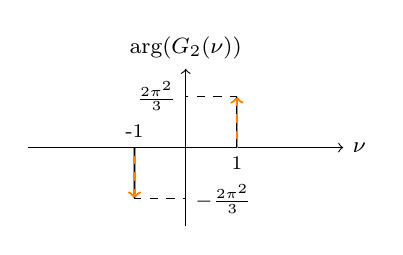
\begin{tikzpicture}
\draw[->] (-2,0)--(2,0) node[right]{\footnotesize{$\nu$}};
\draw[->] (0,-1)--(0,1) node[above]{\footnotesize{$\text{arg}(G_2(\nu))$}};
\draw[->,orange,thick] (-0.65,0)--(-0.65,-0.65) ;
\draw[->,orange,thick] (0.65,0)--(0.65,0.65) ;
\draw[dashed] (-0.65,0)node[above]{\scriptsize -1} --(-0.65,-0.65)--(0,-0.65)node[right]{\scriptsize $-\frac{2\pi^2}{3}$} ;
\draw[dashed] (0.65,0)node[below]{\scriptsize 1} --(0.65,0.65)--(0,0.65)node[left]{\scriptsize $\frac{2\pi^2}{3}$} ;
\end{tikzpicture}
\end{center}

}

\end{columns}

\end{frame}

\begin{frame}
\frametitle{Transformée  de Fourier : Spectre}
La \textbf{phase} a son importance... \\
\vspace{0.3cm}
\small{Si on prend  $g_3(t) = 0.55\cos(2 t) + 0.45 \cos(4 t)$... (on retire le déphasage de $\cos(4 t)$) }\\
\vspace{0.3cm}
\begin{columns}
\column{60mm}
\only<2->{



\begin{center}
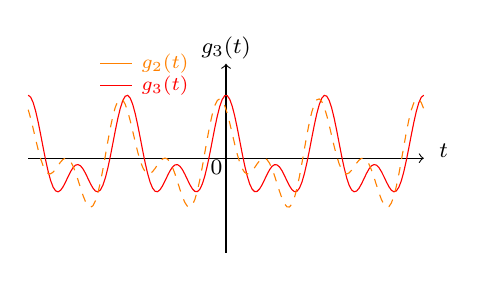
\begin{tikzpicture}
	\begin{scope}[scale=0.4]
	\draw[->] (-6.28,0)-- (6.28,0);
\draw (-0.3,-0.3) node {\footnotesize{0}};
\draw[->] (0,-3)-- (0,3);
\draw (2.2*pi,0.25) node {\footnotesize{$t$}};
\draw (0,3.5) node {\footnotesize{$g_3(t)$}};

	\draw[domain=-6.28:6.28,color=red,samples=160] plot (\x,{2*(0.55*cos(2*\x r)+ 0.45*cos(2*2*\x r))});
	
		\draw[domain=-6.28:6.28,dashed,color=orange,samples=160] plot (\x,{2*(0.55*cos(2*\x r)+ 0.45*cos(2*2*(\x+3.14/12) r))});
		
		\draw[orange] (-4,3)--(-3,3)node[right] {\scriptsize $g_2(t)$};
		\draw[red] (-4,2.3)--(-3,2.3)node[right] {\scriptsize $g_3(t)$};
	\end{scope}
	\end{tikzpicture}
\end{center}


\only<4->
{
Le déphasage $\cos(4t)$  change la forme du signal en impactant UNIQUEMENT la phase 
}

\column{60mm}
\only<3->{
\begin{center}
\begin{tikzpicture}
\draw[->] (-2.5,0)--(2.5,0) node[right]{\footnotesize{$\nu$}};
\draw[->] (0,-1)--(0,1) node[above]{ \footnotesize{$|G_3(\nu)|$}};
\draw[->,red,thick] (-1,0) node[below]{\scriptsize $-1/\pi$}--(-1,0.55) ;
\draw[->,red,thick] (1,0) node[below]{\scriptsize $1/\pi$}--(1,0.55) ;
\draw[->,red,thick] (-2,0) node[below]{\scriptsize $-2/\pi$}--(-2,0.225) ;
\draw[->,red,thick] (2,0) node[below]{\scriptsize $2/\pi$}--(2,0.225) ;
\end{tikzpicture}
\end{center}
\vspace{0cm}
\begin{center}
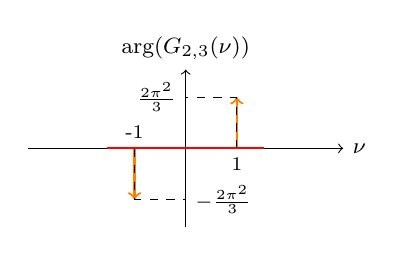
\begin{tikzpicture}
\draw[->] (-2,0)--(2,0) node[right]{\footnotesize{$\nu$}};
\draw[->] (0,-1)--(0,1) node[above]{\footnotesize{$\text{arg}(G_{2,3}(\nu))$}};
\draw[->,orange,thick] (-0.65,0)--(-0.65,-0.65) ;
\draw[->,orange,thick] (0.65,0)--(0.65,0.65) ;
\draw[dashed] (-0.65,0)node[above]{\scriptsize -1} --(-0.65,-0.65)--(0,-0.65)node[right]{\scriptsize $-\frac{2\pi^2}{3}$} ;
\draw[dashed] (0.65,0)node[below]{\scriptsize 1} --(0.65,0.65)--(0,0.65)node[left]{\scriptsize $\frac{2\pi^2}{3}$} ;
\draw[red,thick] (-1,0) --(1,0) ;
\end{tikzpicture}
\end{center}
}
} 
\end{columns}
\vspace{0.3cm}

\end{frame}

\begin{frame}
\frametitle{Forme des spectres en amplitude}
\begin{columns}
\column{60mm}
\begin{center}
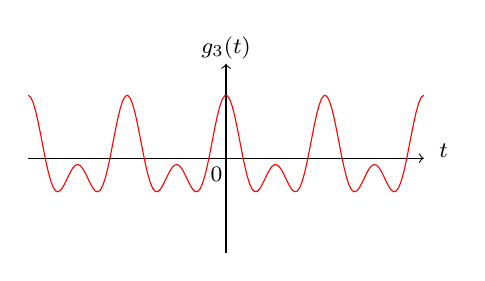
\begin{tikzpicture}
	\begin{scope}[scale=0.4]
	\draw[->] (-6.28,0)-- (6.28,0);
\draw (-0.3,-0.5) node {\footnotesize{0}};
\draw[->] (0,-3)-- (0,3);
\draw (2.2*pi,0.25) node {\footnotesize{$t$}};
\draw (0,3.5) node {\footnotesize{$g_3(t)$}};

	\draw[domain=-6.28:6.28,color=red,samples=160] plot (\x,{2*(0.55*cos(2*\x r)+ 0.45*cos(2*2*\x r))});
	
		
	\end{scope}
	\end{tikzpicture}
\end{center}
\column{60mm}
\begin{center}
\begin{tikzpicture}
\draw[->] (-2.5,0)--(2.5,0) node[right]{\footnotesize{$\nu$}};
\draw[->] (0,-1)--(0,1) node[above]{ \footnotesize{$|G_3(\nu)|$}};
\draw[->,red,thick] (-1,0) node[below]{\scriptsize $-1/\pi$}--(-1,0.55) ;
\draw[->,red,thick] (1,0) node[below]{\scriptsize $1/\pi$}--(1,0.55) ;
\draw[->,red,thick] (-2,0) node[below]{\scriptsize $-2/\pi$}--(-2,0.225) ;
\draw[->,red,thick] (2,0) node[below]{\scriptsize $2/\pi$}--(2,0.225) ;
\end{tikzpicture}
\end{center}
\end{columns}
\vspace{0.5cm}
\small{\underline{Analyse de Fourier}: 
\begin{itemize}
\item Signal périodique = somme de sinusoïdes
\item somme de sinusoïdes = spectre de raies
\end{itemize}}
\center
Donc \textbf{Signal périodique = Spectre de raies}
\end{frame}

\begin{frame}
\frametitle{Résumé Séance 1}
\begin{enumerate}
\item Signal: concept et types
\vspace{0.3cm}
\item Outils mathématiques pour le traitement du signal 
\vspace{0.3cm}
\item Transformée de Laplace 
\vspace{0.3cm}
\item Transformée de Fourier 
\end{enumerate}
\end{frame}

\subsection{Concepts utile dans le domaine de Fourier}

\begin{frame}
\frametitle{Choses à savoir sur la Transformée de Fourier}
Il y a des petites "lois" qu'il peut être utile d'avoir à l'esprit lorsqu'on manipule des fonctions et leurs spectres...\\

\vspace{0.1cm}
\only<2->
{
1a.\textbf{ Extension temporelle faible = Extension fréquentielle forte}
}

\only<3->{
\begin{center}
\begin{tikzpicture}
\draw[->] (-2,0)--(2,0) node[right]{$t$};
\draw[->] (0,-1)--(0,1) node[above]{$f(t)$};
\draw[thick,blue] (-2,0)--(0,0)--(0,1)--(0,0)--(2,0);

\begin{scope}[xshift=6cm]
\draw[->] (-2,0)--(2,0) node[right]{$\nu$};
\draw[->] (0,-1)--(0,1) node[above]{$F(\nu)$};
\draw[thick,blue] (-2,0.5)--(2,0.5);
\end{scope}
\end{tikzpicture}
\end{center}
}

\only<4->
{
1b.\textbf{ Extension temporelle forte = Extension fréquentielle faible}
}

\only<4->{
\begin{center}
\begin{tikzpicture}
\draw[->] (-2,0)--(2,0) node[right]{$t$};
\draw[->] (0,-1)--(0,1) node[above]{$f(t)$};
\draw[thick,blue] (-2,0.5)--(2,0.5);

\begin{scope}[xshift=6cm]
\draw[->] (-2,0)--(2,0) node[right]{$\nu$};
\draw[->] (0,-1)--(0,1) node[above]{$F(\nu)$};
\draw[thick,blue] (-2,0)--(0,0)--(0,1)--(0,0)--(2,0);
\end{scope}
\end{tikzpicture}
\end{center}
}

\end{frame} 

\begin{frame}
\frametitle{Choses à savoir sur la Transformée de Fourier}
2. Périodicité temporelle et spectre 


\only<2->{
\begin{tikzpicture}
\draw[->] (2.5,0) node[below] {0} -- (2.5,1.5)node[above] {$e(t)$};
\draw[->] (0,0)-- (5,0) node[right] {$t$};

\draw[thick,blue] (2,0)--(2.25,0)--(2.25,1)--(2.75,1)--(2.75,0)--(3,0);

\begin{scope}[xshift=1cm]
\draw[thick,blue] (2,0)--(2.25,0)--(2.25,1)--(2.75,1)--(2.75,0)--(3,0);
\draw[dashed,black] (2.5,0) node[below]{$T$}--(2.5,1);
\end{scope}

\begin{scope}[xshift=2cm]
\draw[thick,blue] (2,0)--(2.25,0)--(2.25,1)--(2.75,1)--(2.75,0)--(3,0);
\end{scope}


\begin{scope}[xshift=-1cm]
\draw[thick,blue] (2,0)--(2.25,0)--(2.25,1)--(2.75,1)--(2.75,0)--(3,0);
\end{scope}

\begin{scope}[xshift=-2cm]
\draw[thick,blue] (2,0)--(2.25,0)--(2.25,1)--(2.75,1)--(2.75,0)--(3,0);
\end{scope}



\begin{scope}[xshift=7cm]
\draw[->] (2.5,0) node[below] {0} -- (2.5,1.5)node[above] {$E(\nu)$};
\draw[->] (0,0)-- (5,0) node[right] {$\nu$};
\draw[ domain=0.1:4.9,color=blue,samples=24] plot[ycomb] (\x,{80*abs(sin(5*3.14*\x r -5*3.14*2.5r )/(5*3.14*\x r-5*3.14*2.5 r))});
\draw[<->] (3.25,-0.3)--(3.45,-0.3) node[below left] {$\frac{1}{T}$};
\end{scope}
\end{tikzpicture}
}

\only<3->{
\begin{tikzpicture}
\draw[->] (2.5,0) node[below] {0} -- (2.5,1.5)node[above] {$e(t)$};
\draw[->] (0,0)-- (5,0) node[below right] {$t$};

\draw[thick,blue] (1,0)--(2.25,0)--(2.25,1)--(2.75,1)--(2.75,0)--(4,0);


\begin{scope}[xshift=2cm]
\draw[thick,blue] (1,0)--(2.25,0)--(2.25,1)--(2.75,1)--(2.75,0)--(3,0);
\end{scope}


\begin{scope}[xshift=-2cm]
\draw[thick,blue] (2,0)--(2.25,0)--(2.25,1)--(2.75,1)--(2.75,0)--(4,0);
\end{scope}



\begin{scope}[xshift=7cm]
\draw[->] (2.5,0) node[below] {0} -- (2.5,1.5)node[above] {$E(\nu)$};
\draw[->] (0,0)-- (5,0) node[right] {$\nu$};
\draw[ domain=0.1:4.9,color=blue,samples=96] plot[ycomb] (\x,{80*abs(sin(5*3.14*\x r -5*3.14*2.5r )/(5*3.14*\x r-5*3.14*2.5 r))});
%\draw[<->] (3.25,-0.3)--(3.45,-0.3) node[below left] {$\frac{1}{T}$};
\end{scope}
\end{tikzpicture}
}

\only<4->{
Pertinent lorsqu'il est question d'échantillonnage...
}
\end{frame}
\end{document}
